\documentclass[12pt]{article}
\usepackage{verbatim}
\usepackage[dvips]{epsfig}
\usepackage{color}
\usepackage{url}
\usepackage[colorlinks=true]{hyperref}

\begin{document}

\section*{GENESIS: Documentation}

{\bf Related Documentation:}
% start: userdocs-tag-replace-items related-do-nothing
% end: userdocs-tag-replace-items related-do-nothing

\section*{De Schutter: Purkinje Cell Model}

\subsection*{Figure\,4}

\begin{figure}[h]
\centering
   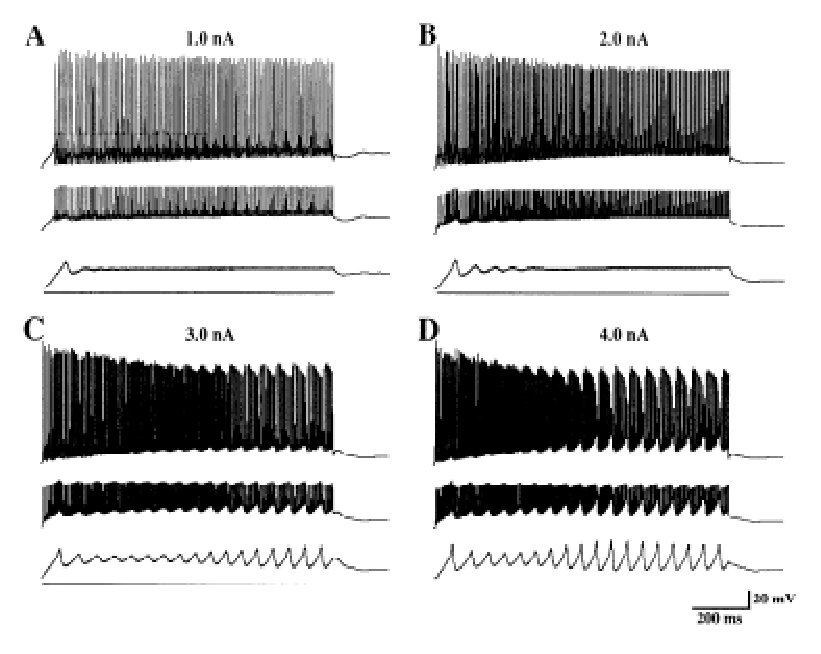
\includegraphics[scale=1]{figures/Fig.1.4.eps}
   \caption{Simulation of current injection in the
soma, model PM9. For each current injection amplitude
(A: 0.5\,nA, B: 1.0\,nA, C: 2.0\,nA, D: 3.0\,
nA) 3 recording sites are shown: the soma (top
trace), the main dendrite (middle trace), and a
spiny dendrite (bottom trace). Bar below traces: duration
of current injection.}
   \label{fig:DS1.4}
\end{figure}

\bibliographystyle{plain}
\bibliography{../tex/bib/g3-refs.bib}

\end{document}
